
\begin{figure}
    \centering
    \begin{fullwidth}
    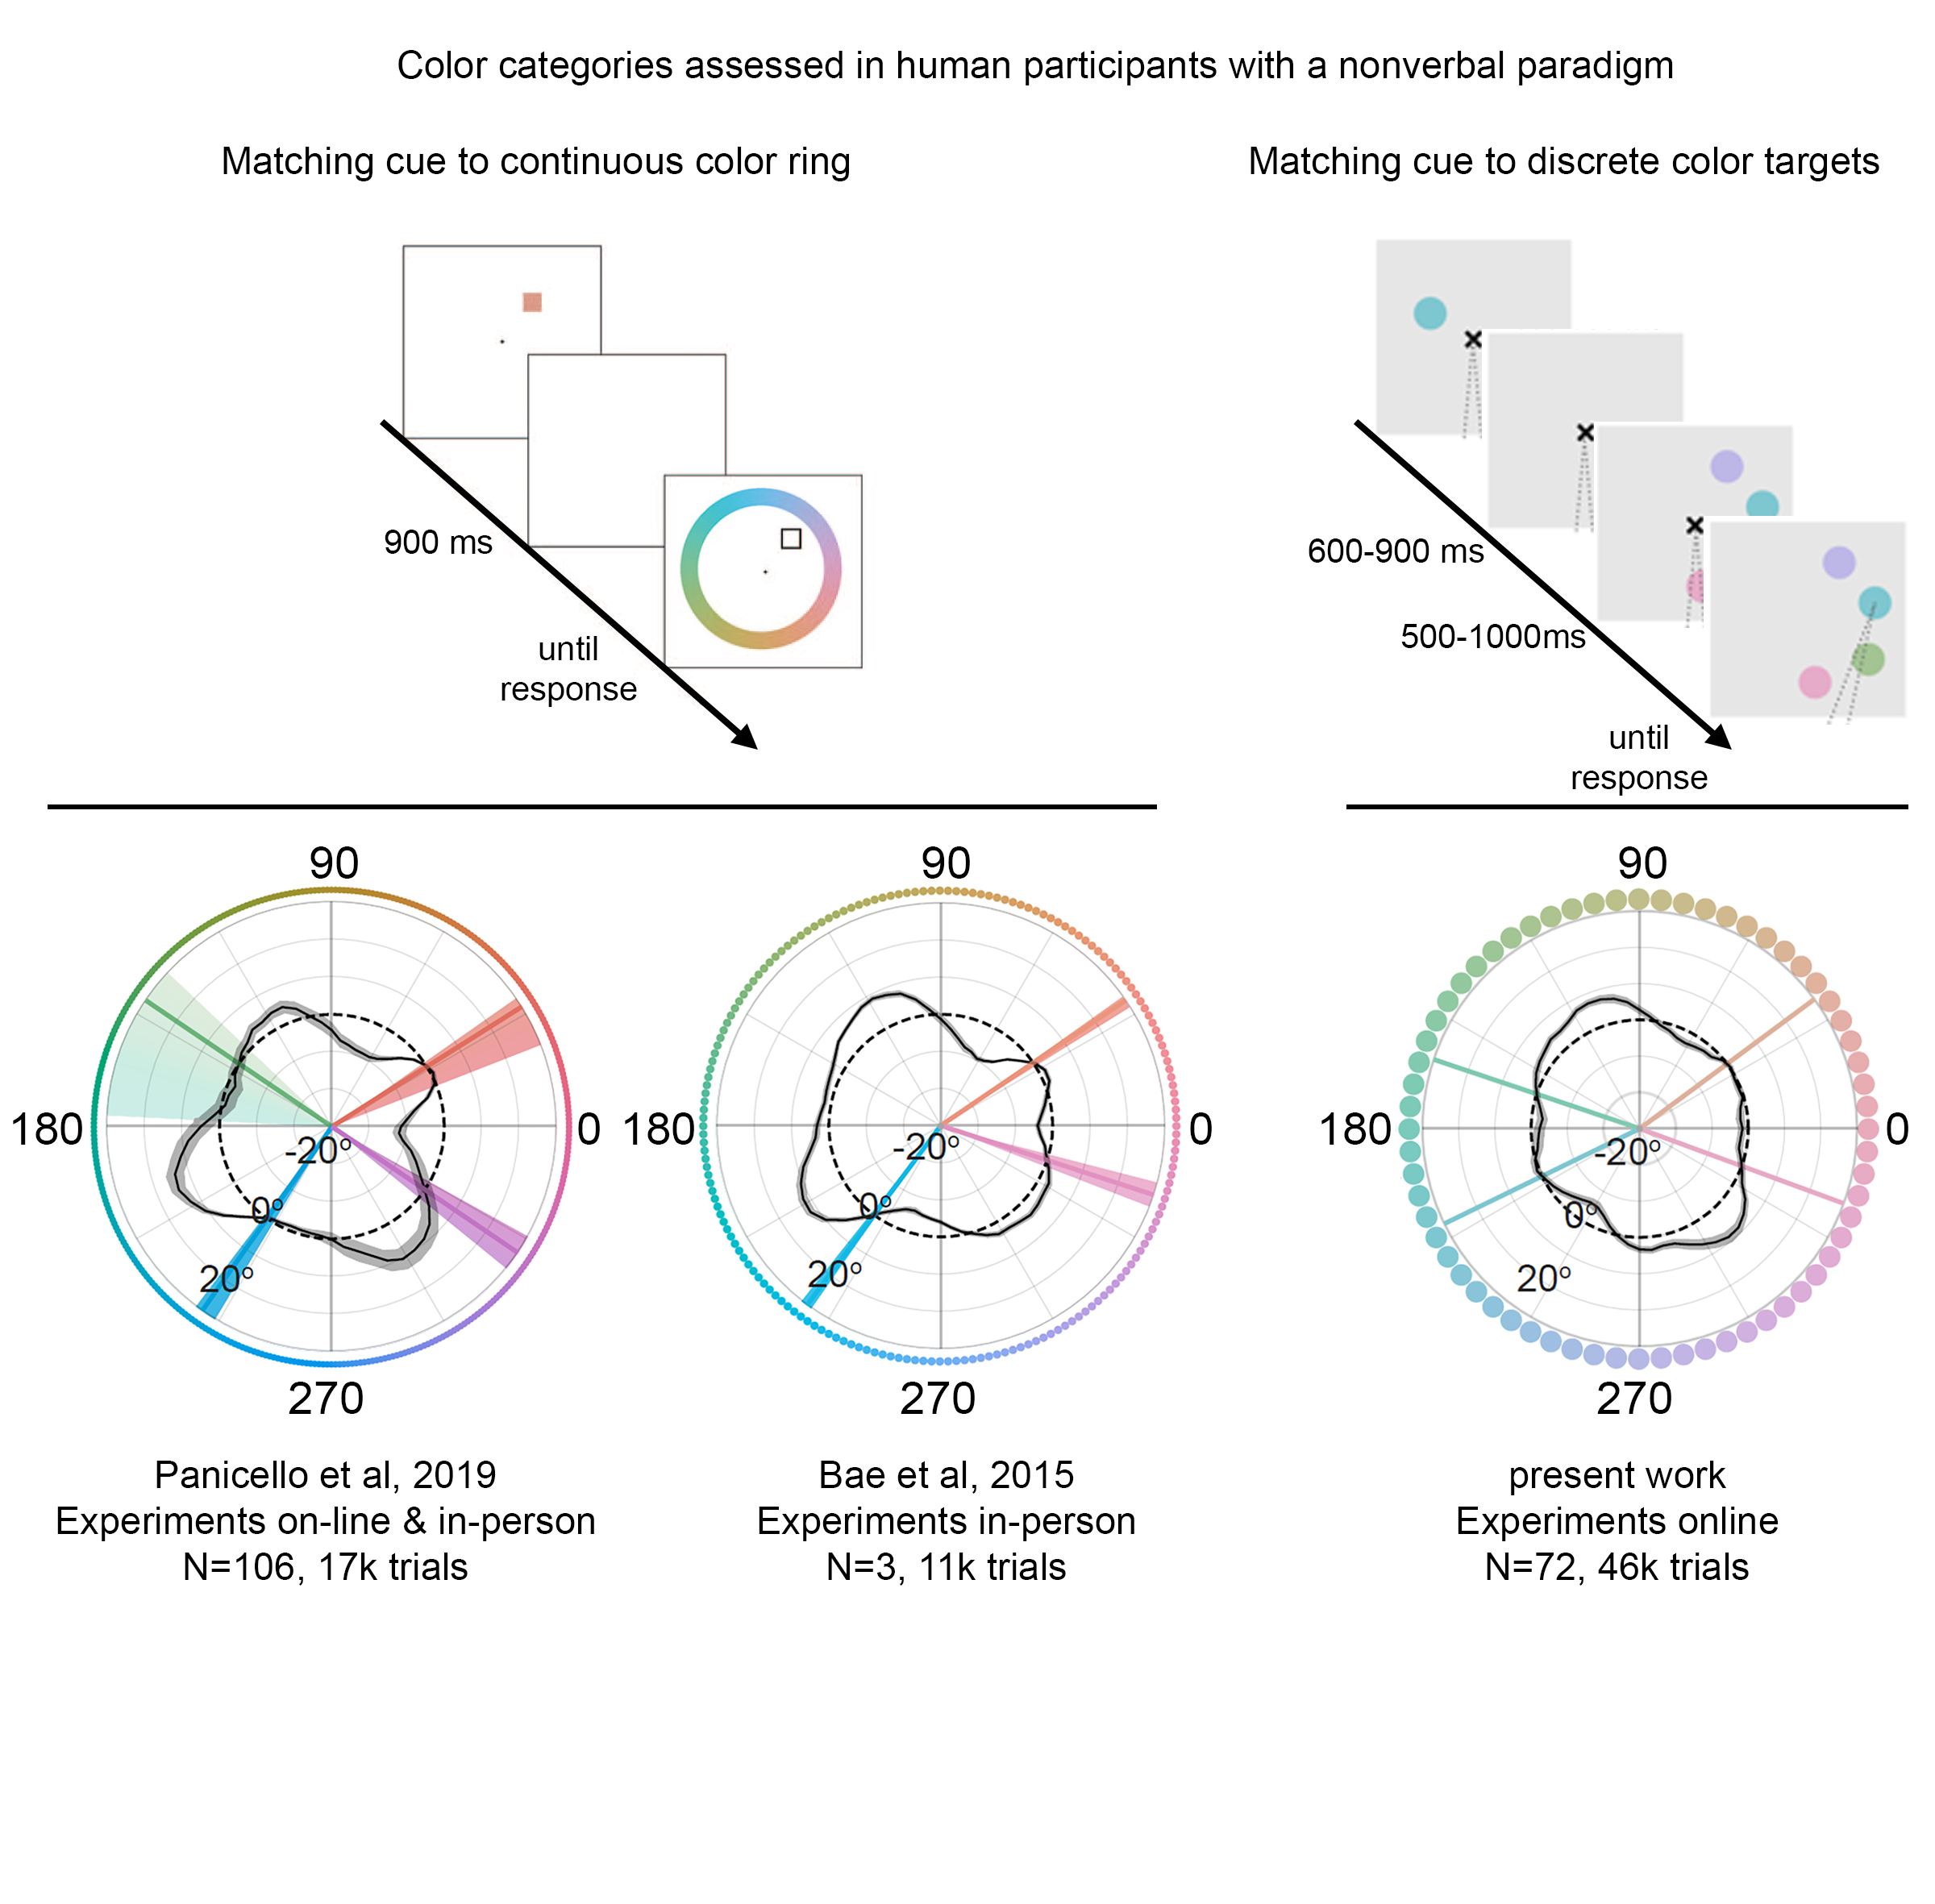
\includegraphics[width=\textwidth+4cm,trim={0 2cm 0 0},clip]{../Figures/flat/SI1_Human.jpg}
    \caption{\textbf{Color categories assessed in human participants with a nonverbal paradigm. }
    Prior work by \citep{bae_why_2015} and \citep{panichello_error-correcting_2019} has used a task in which participants match the color of a cue to a continuous ring of colors; those published results were obtained with a combination of in-person experiments and on-line experiments, and the results are consistent for both kinds of experiments. 
    A mixture-model analysis of the results recovers four color categories, corresponding to blue, green, orange and pink. 
    Note that the data from \citep{bae_why_2015} shown in the figure were from just three participants; those authors confirmed the results in more subjects with a version of the task that omitted the memory delay period (so the cue and the match-option color wheel were presented simultaneously). 
    The present work adapted the paradigm so that the match options were discrete targets, which avoids the risk of reinforcing idiosyncratic biases that arises when using the task in non-human primates, by allowing greater precision (only direct matches are rewarded). 
    In human participants, with experiments conducted online with Amazon Mechanical Turk, the results using the discrete-matching paradigm recover the same number of significant color categories as the continuous-matching paradigm.
    These four categories correspond to the four categories recovered in the prior work, blue, green, orange, pink. 
    We note that the discrete-matching task recovers a trend for a fifth category that would correspond to “purple”; close inspection of the results in Bae et al (2015) also provide evidence of this trend. 
    } 
    \label{fig:Human}
    \end{fullwidth}
\end{figure}

\begin{figure}
    \centering
    \begin{fullwidth}
    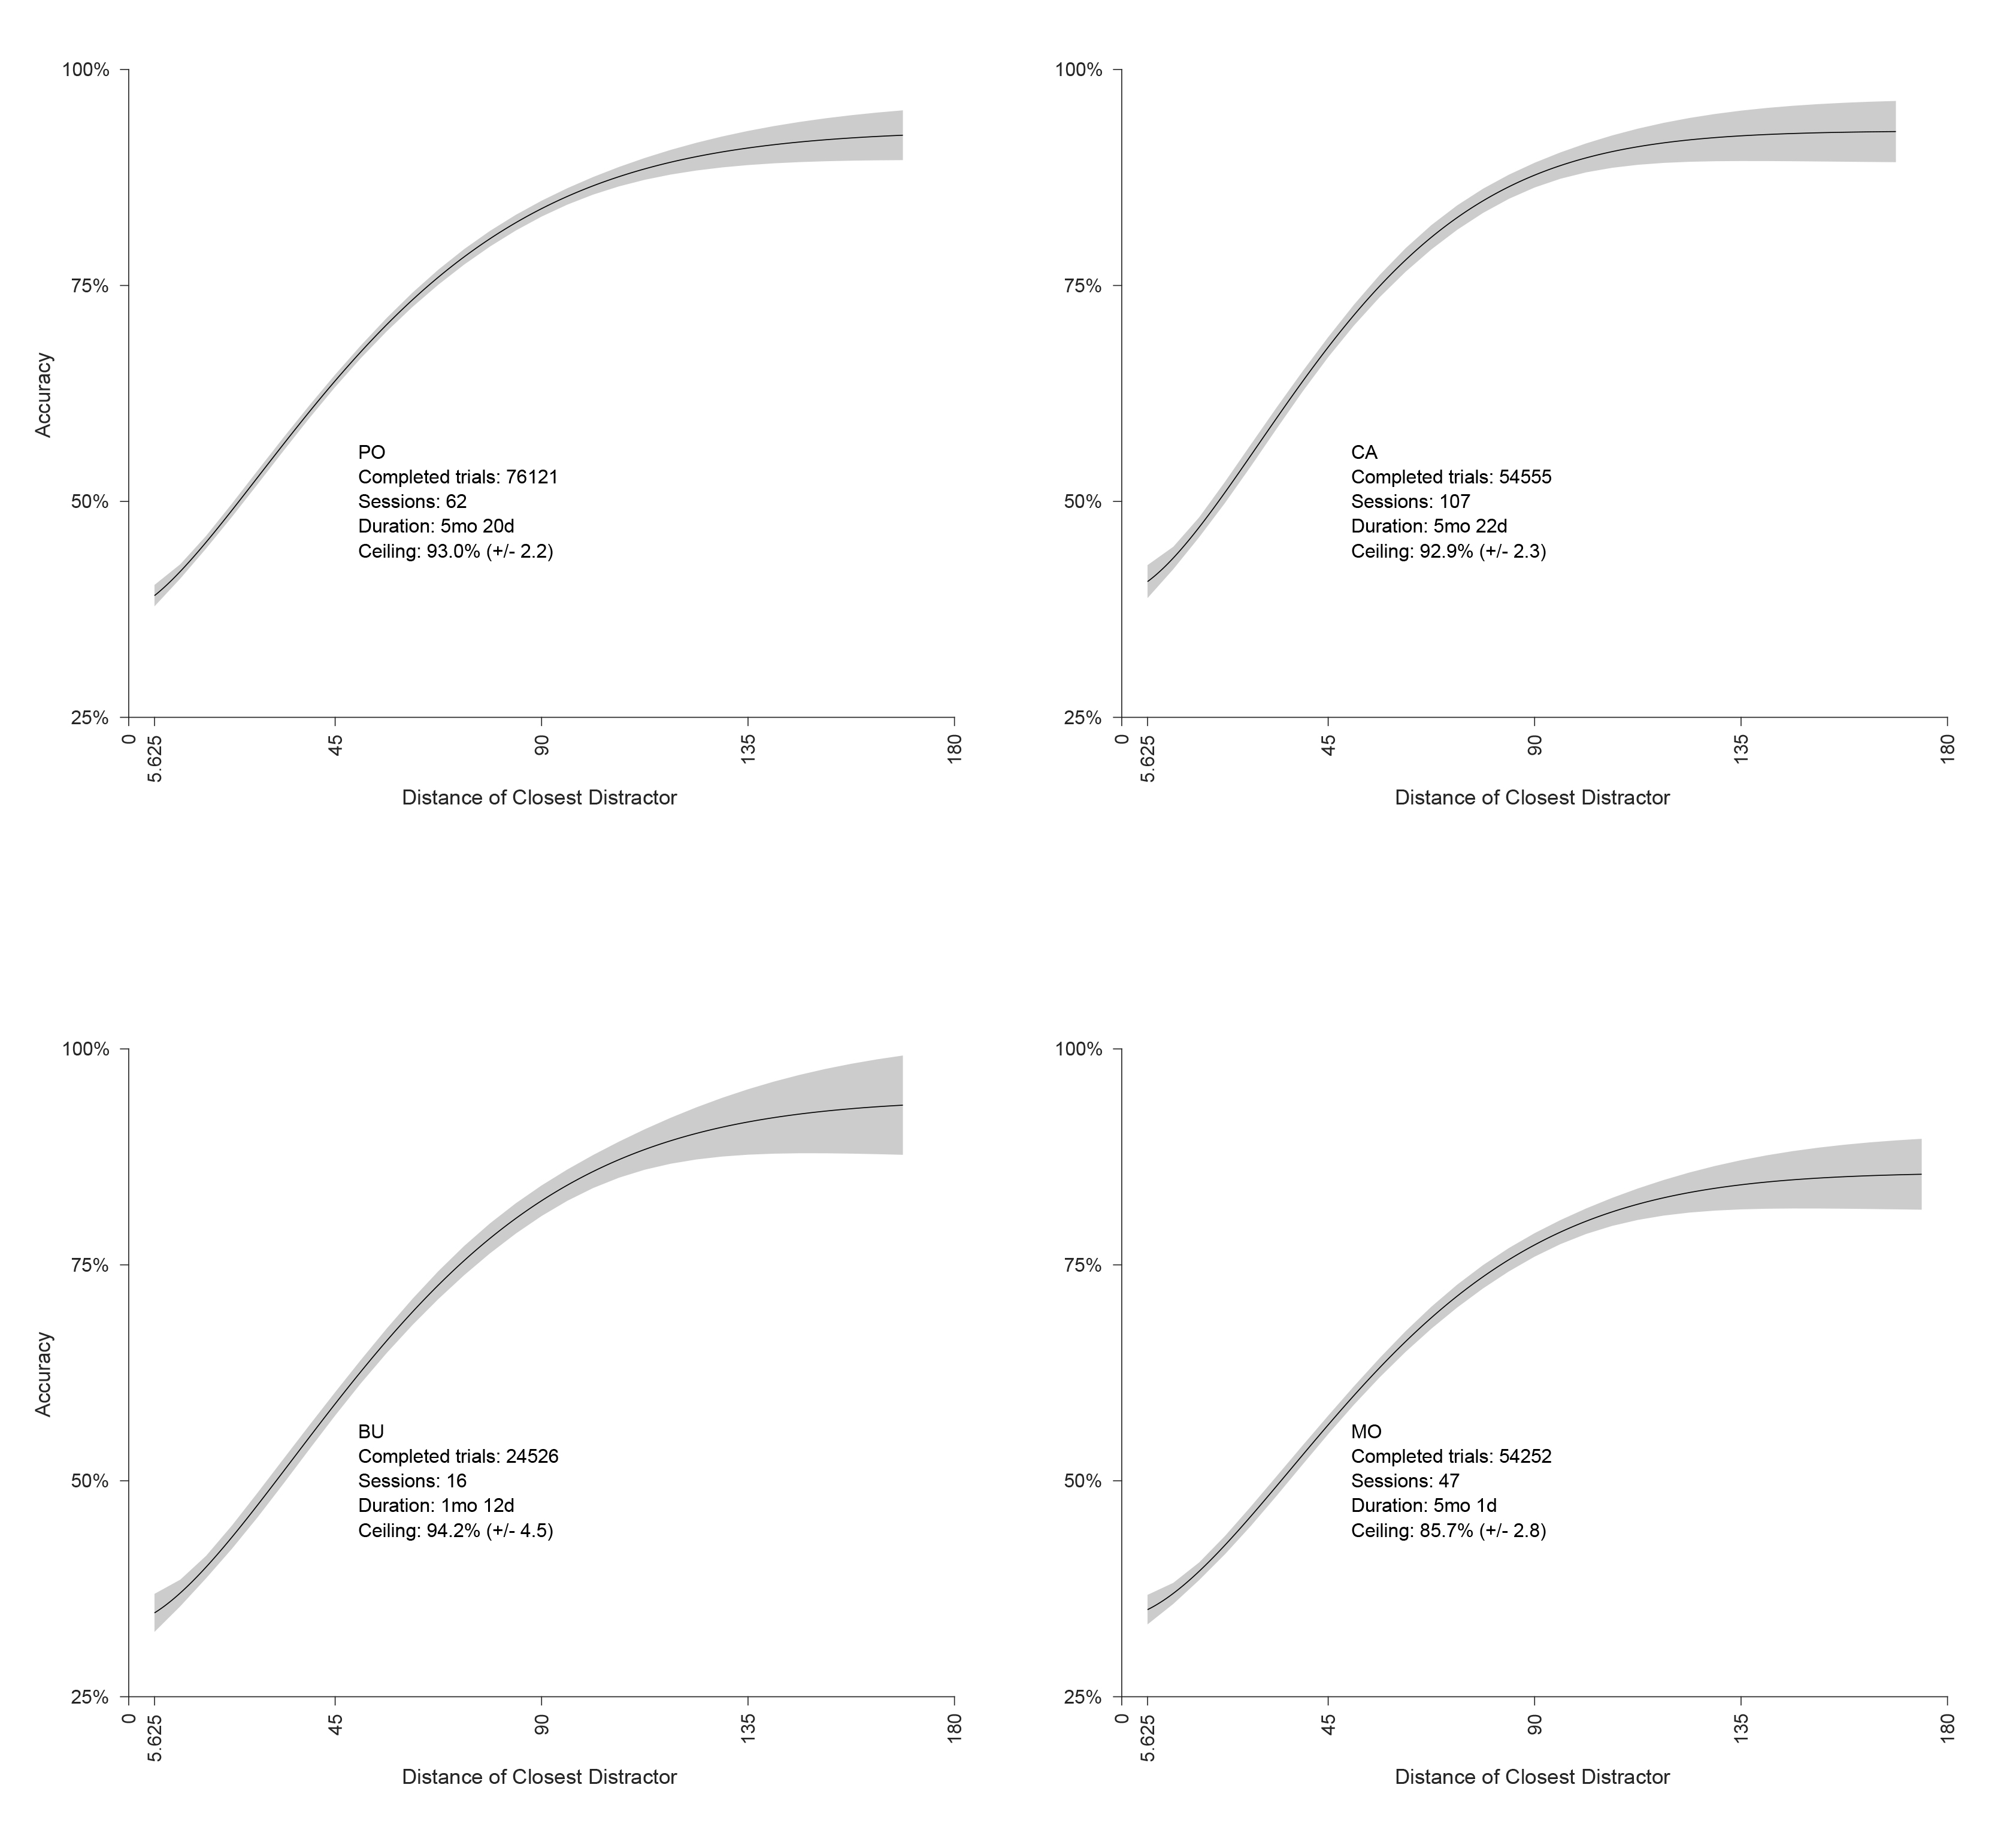
\includegraphics[width=\textwidth+4cm]{../Figures/flat/SI2_psychometric.jpg}
    \caption{\textbf{Psychometric functions for the four individual animals (PO, CA, BU, MO) on the color-matching task illustrated in Figure 1.}
    Completed trials for the four animals were: 76121; 54555; 24526; 54252.
    } 
    \label{fig:IndiDiff}
    \end{fullwidth}
\end{figure}

\begin{figure}
    \centering
    \begin{fullwidth}
    \includegraphics[width=\textwidth+4cm]{../Figures/flat/SI3_MMBreakOut.jpg}
    \caption{\textbf{Gaussian fits from the Mixture Model.}
    Each trace shows the Gaussian fit for one of the 64 target colors used in the color-matching task, as per Equation 1; data averaged over four animals.
    } 
    \label{fig:MMBreakOut}
    \end{fullwidth}
\end{figure}

\begin{figure}
    \centering
    \begin{fullwidth}
    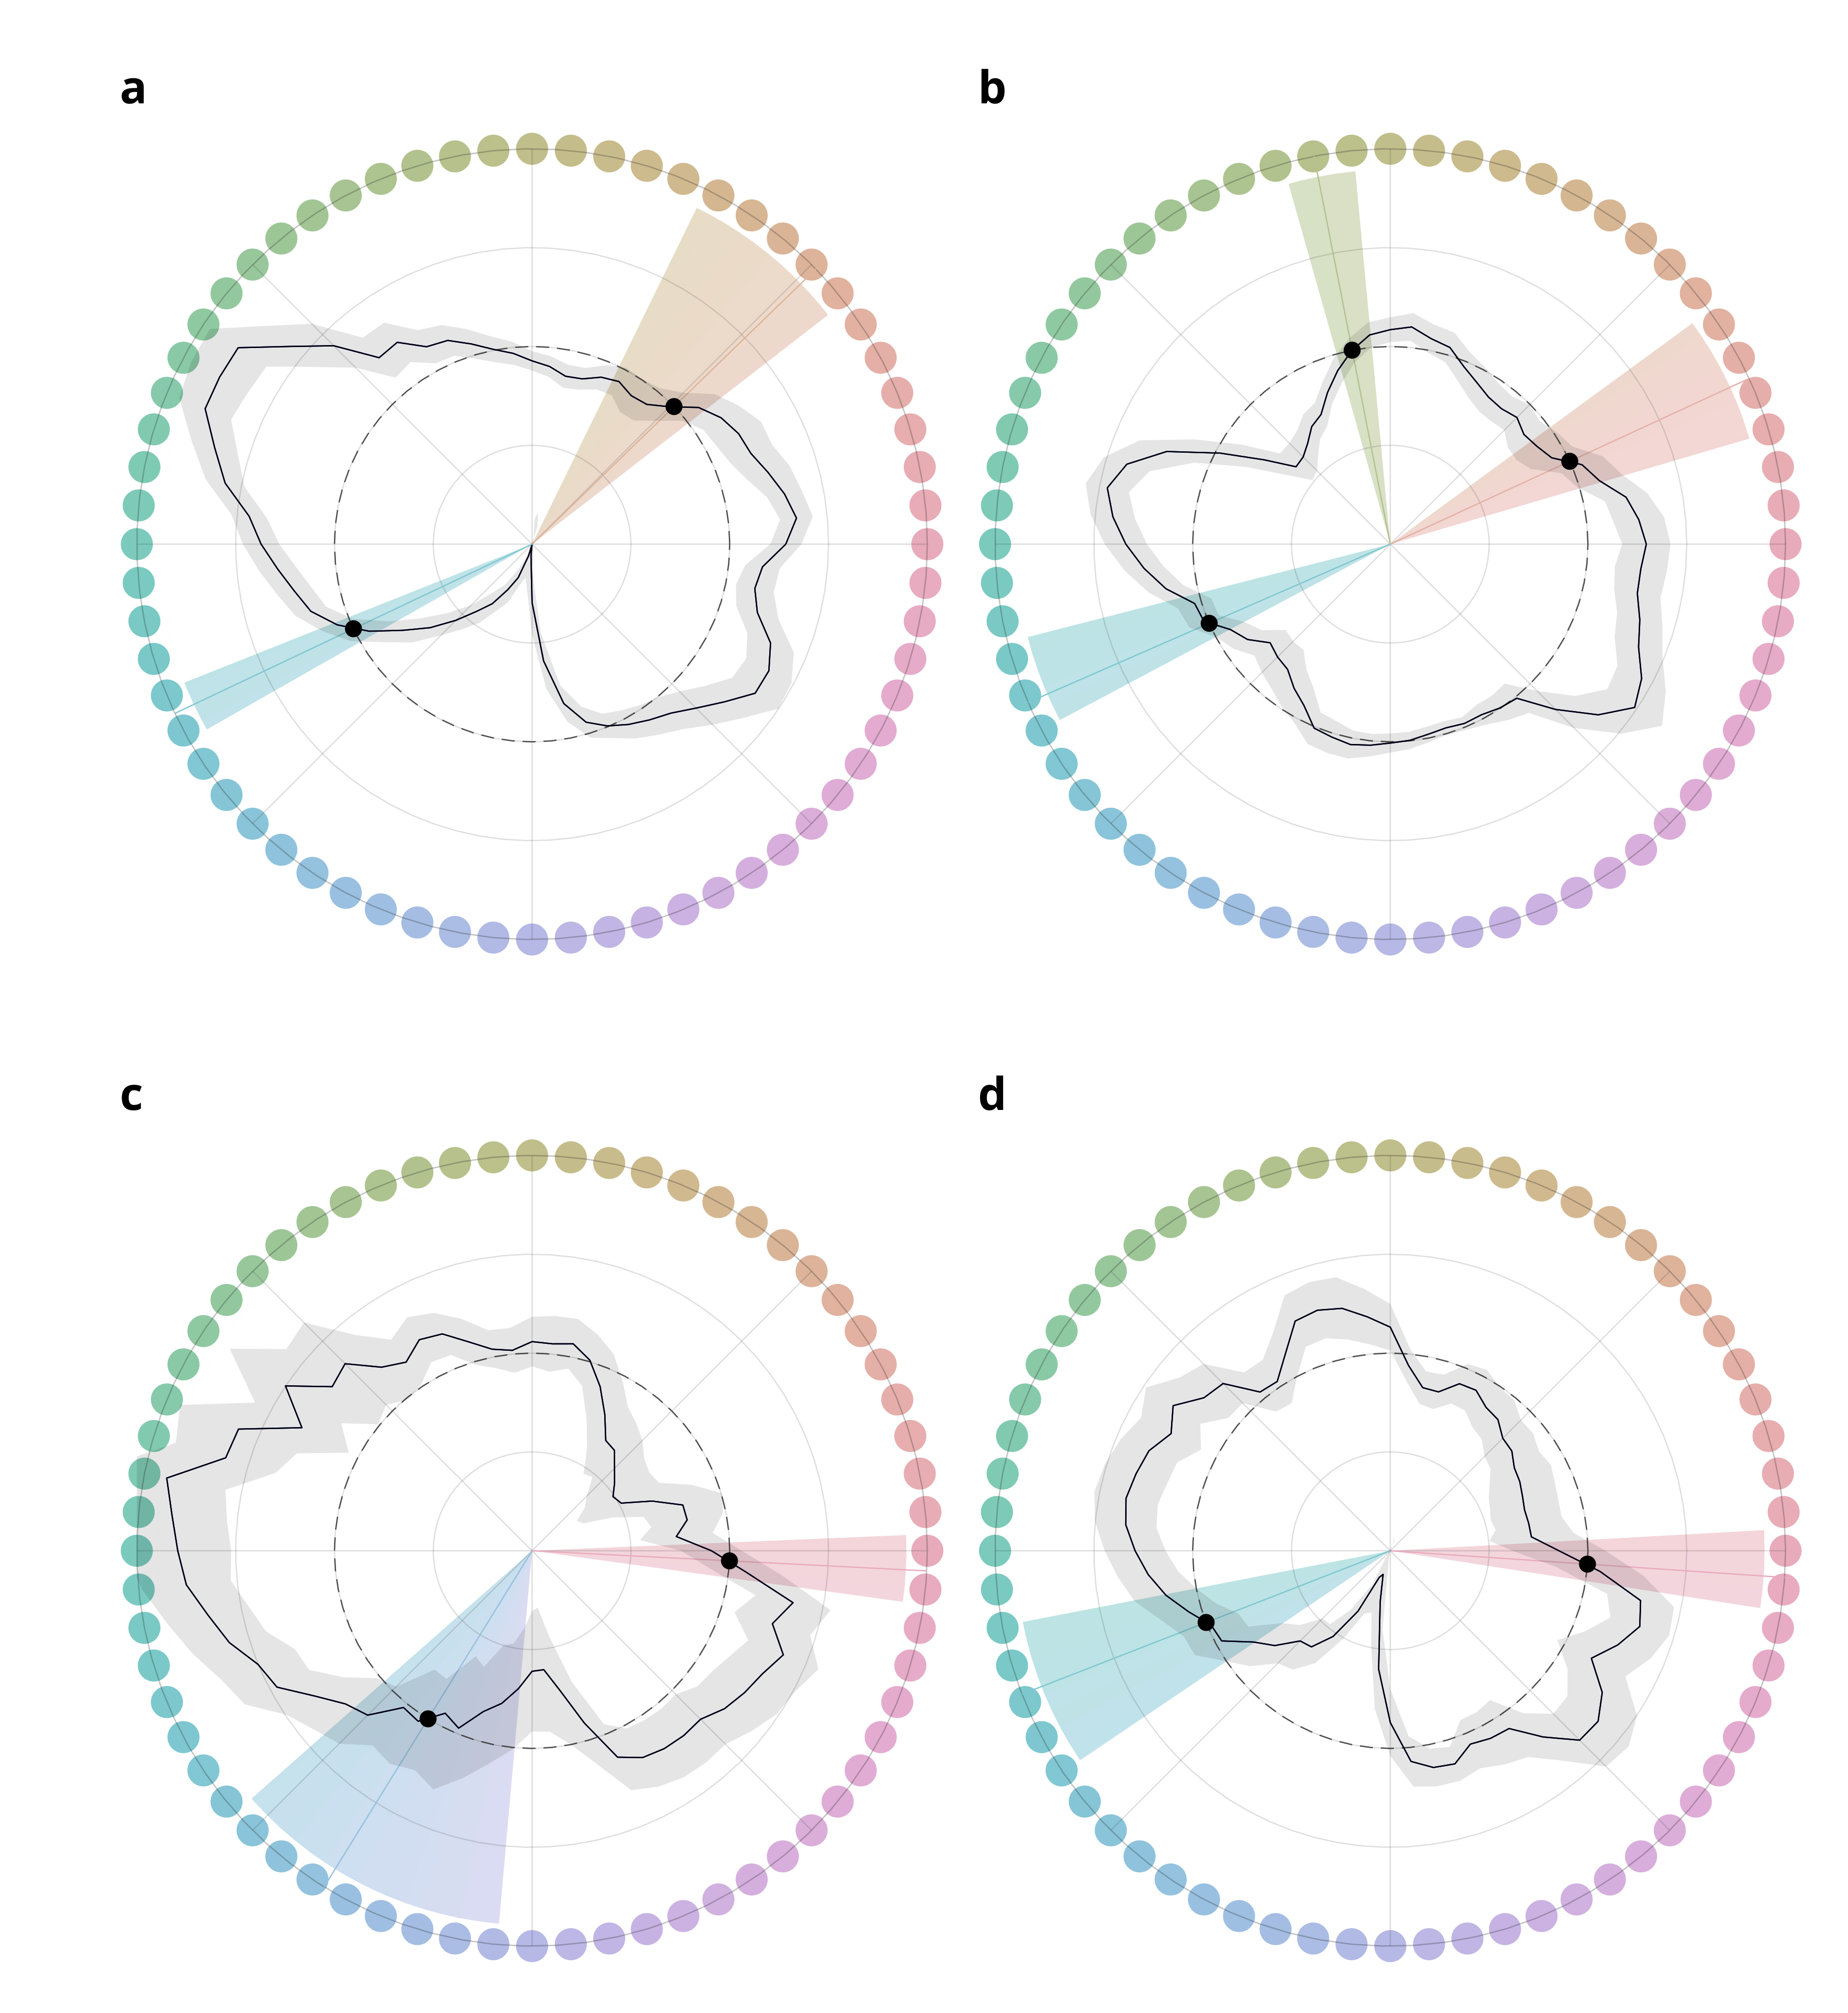
\includegraphics[width=\textwidth+4cm]{../Figures/flat/SI4_MM.jpg}
    \caption{\textbf{Mixture-model analysis of the individual data for the four animals in the color-matching task.}
    Data shown in the same format as Figure 2c; data subsampled to ensure the same amount of data per animal.
    } 
    \label{fig:IndiMM}
    \end{fullwidth}
\end{figure}

\begin{figure}
    \centering
    \begin{fullwidth}
    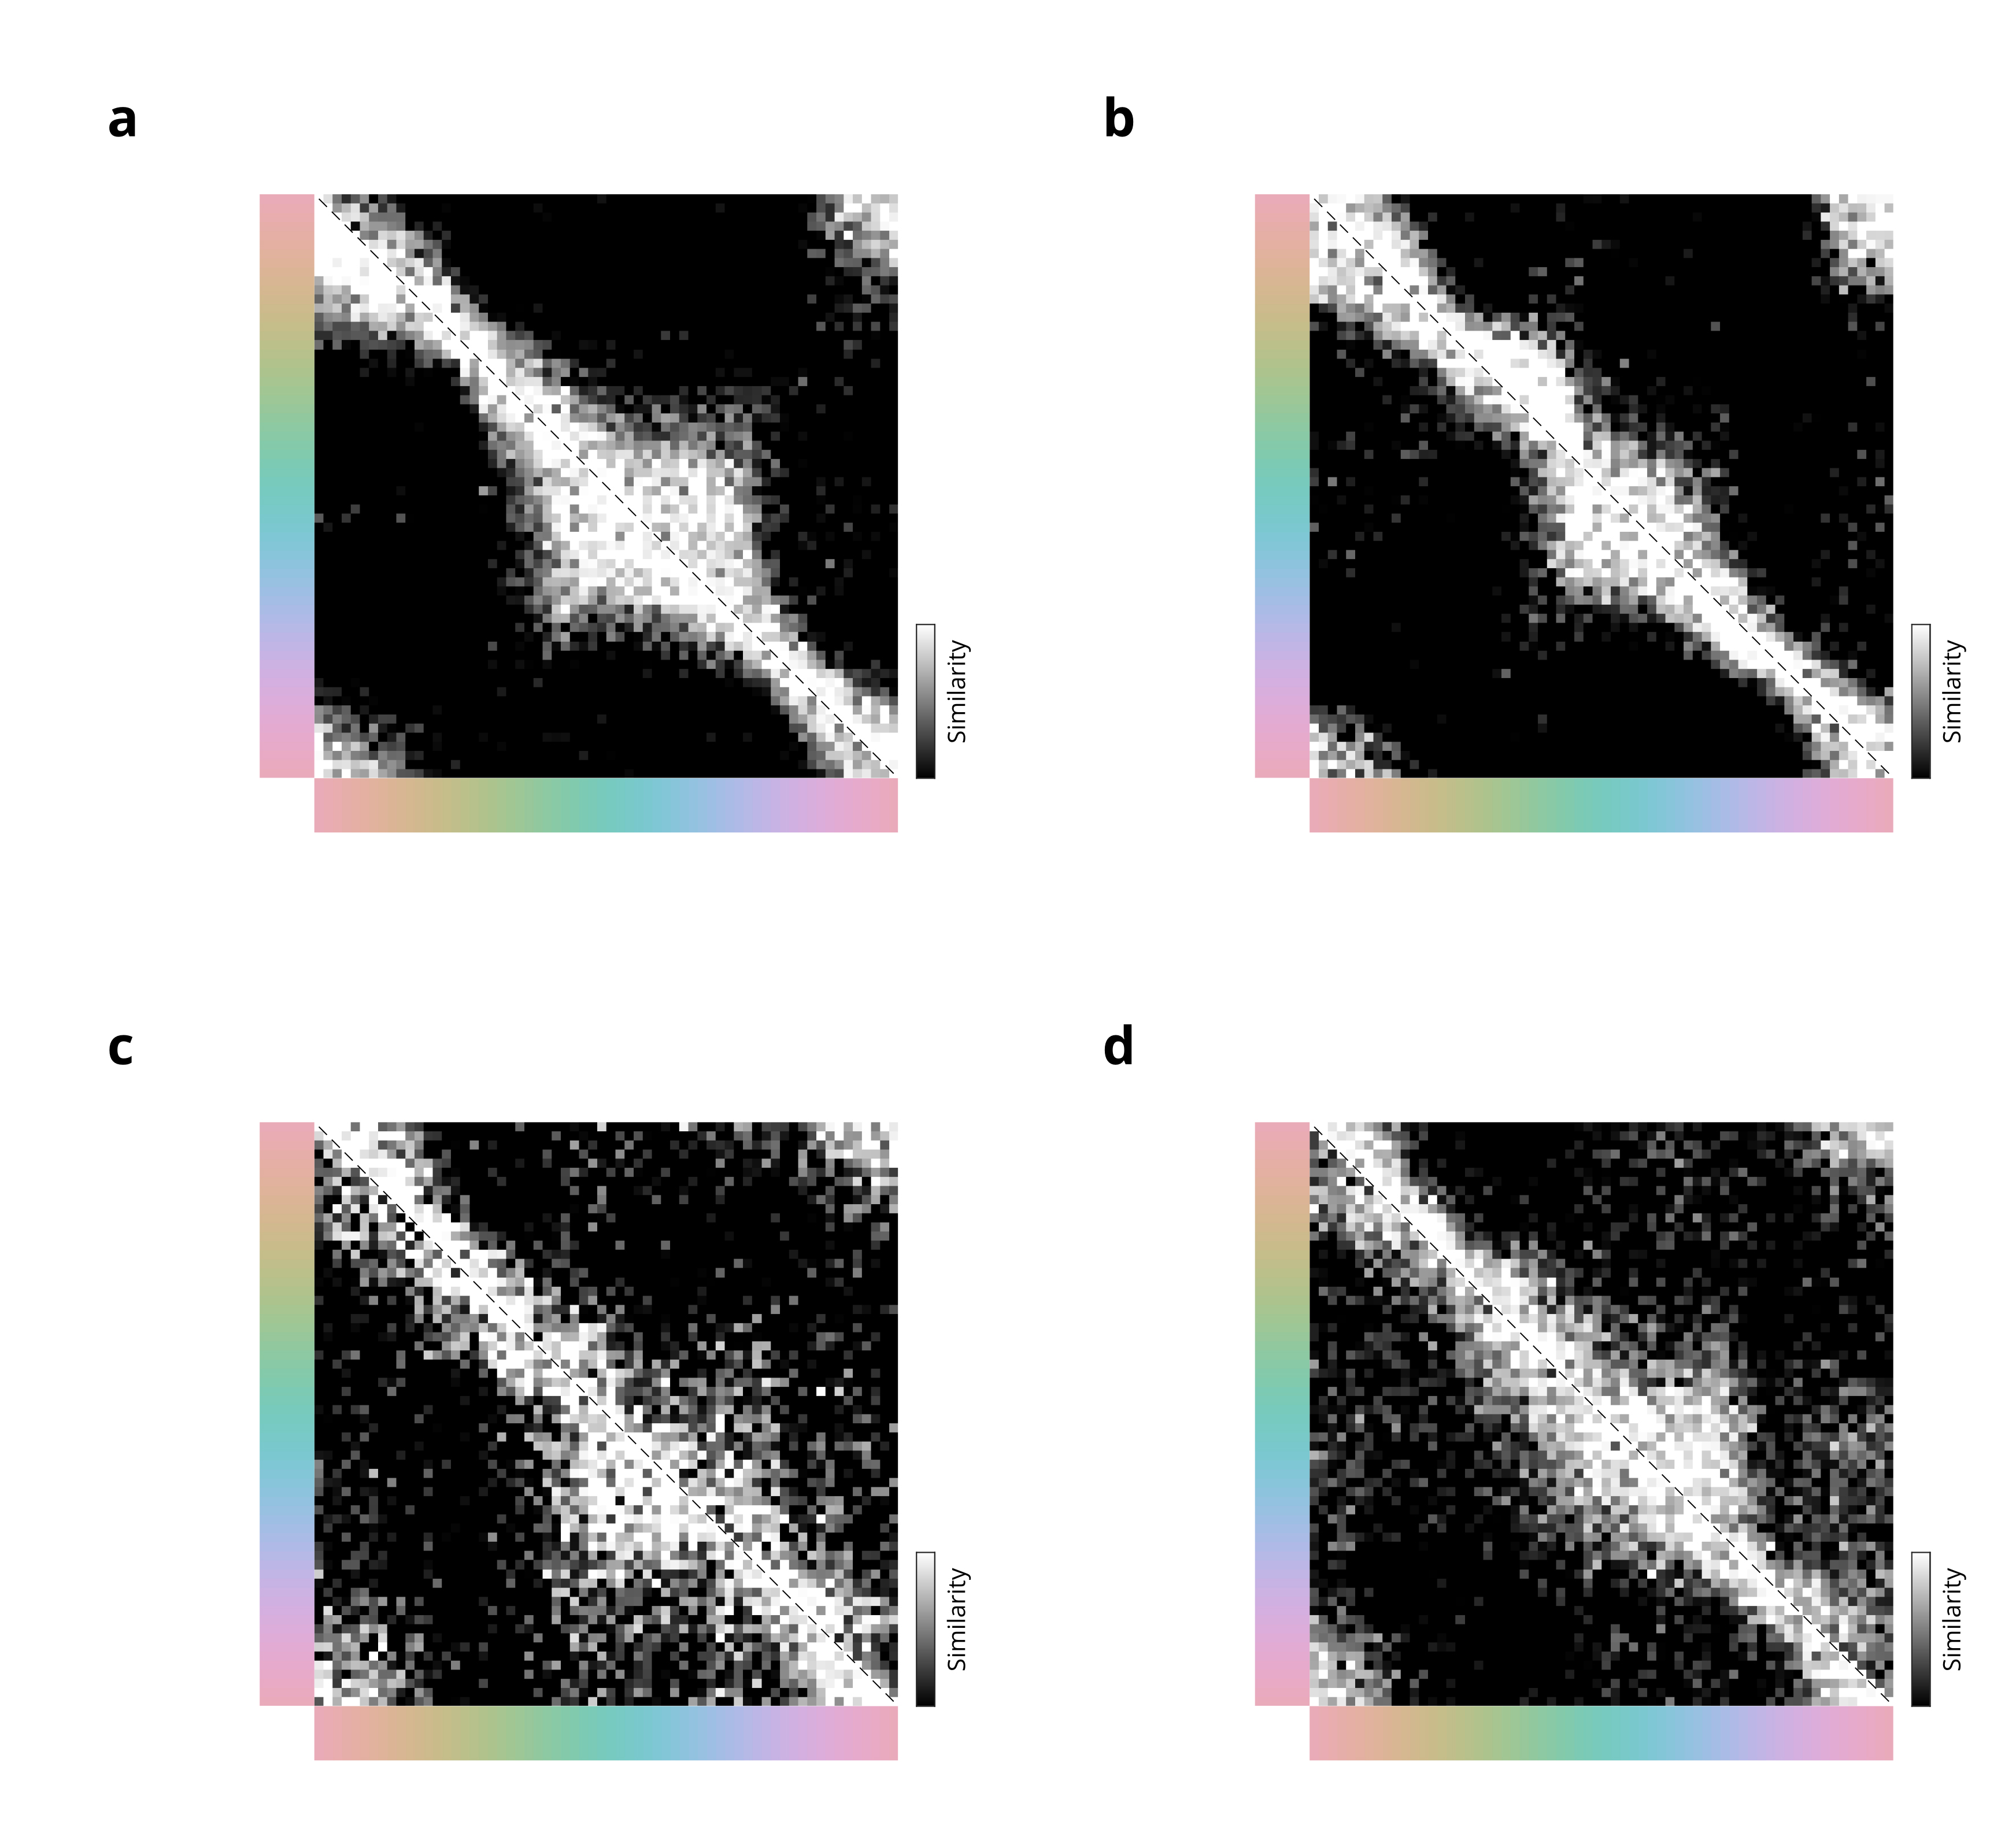
\includegraphics[width=\textwidth+4cm]{../Figures/flat/SI5_IndTCCv.jpg}
    \caption{\textbf{Similarity matrices for free similarity matrix models, fit to individual data.}
    The order of the plots is the same as the order in other figures, PO, CA, BU, MO. See Figure 3ab for data averaged across animals, with data subsamples to ensure the same amount of data per animal.
    } 
    \label{fig:IndiTCC}
    \end{fullwidth}
\end{figure}

\begin{figure}
    \centering
    \begin{fullwidth}
    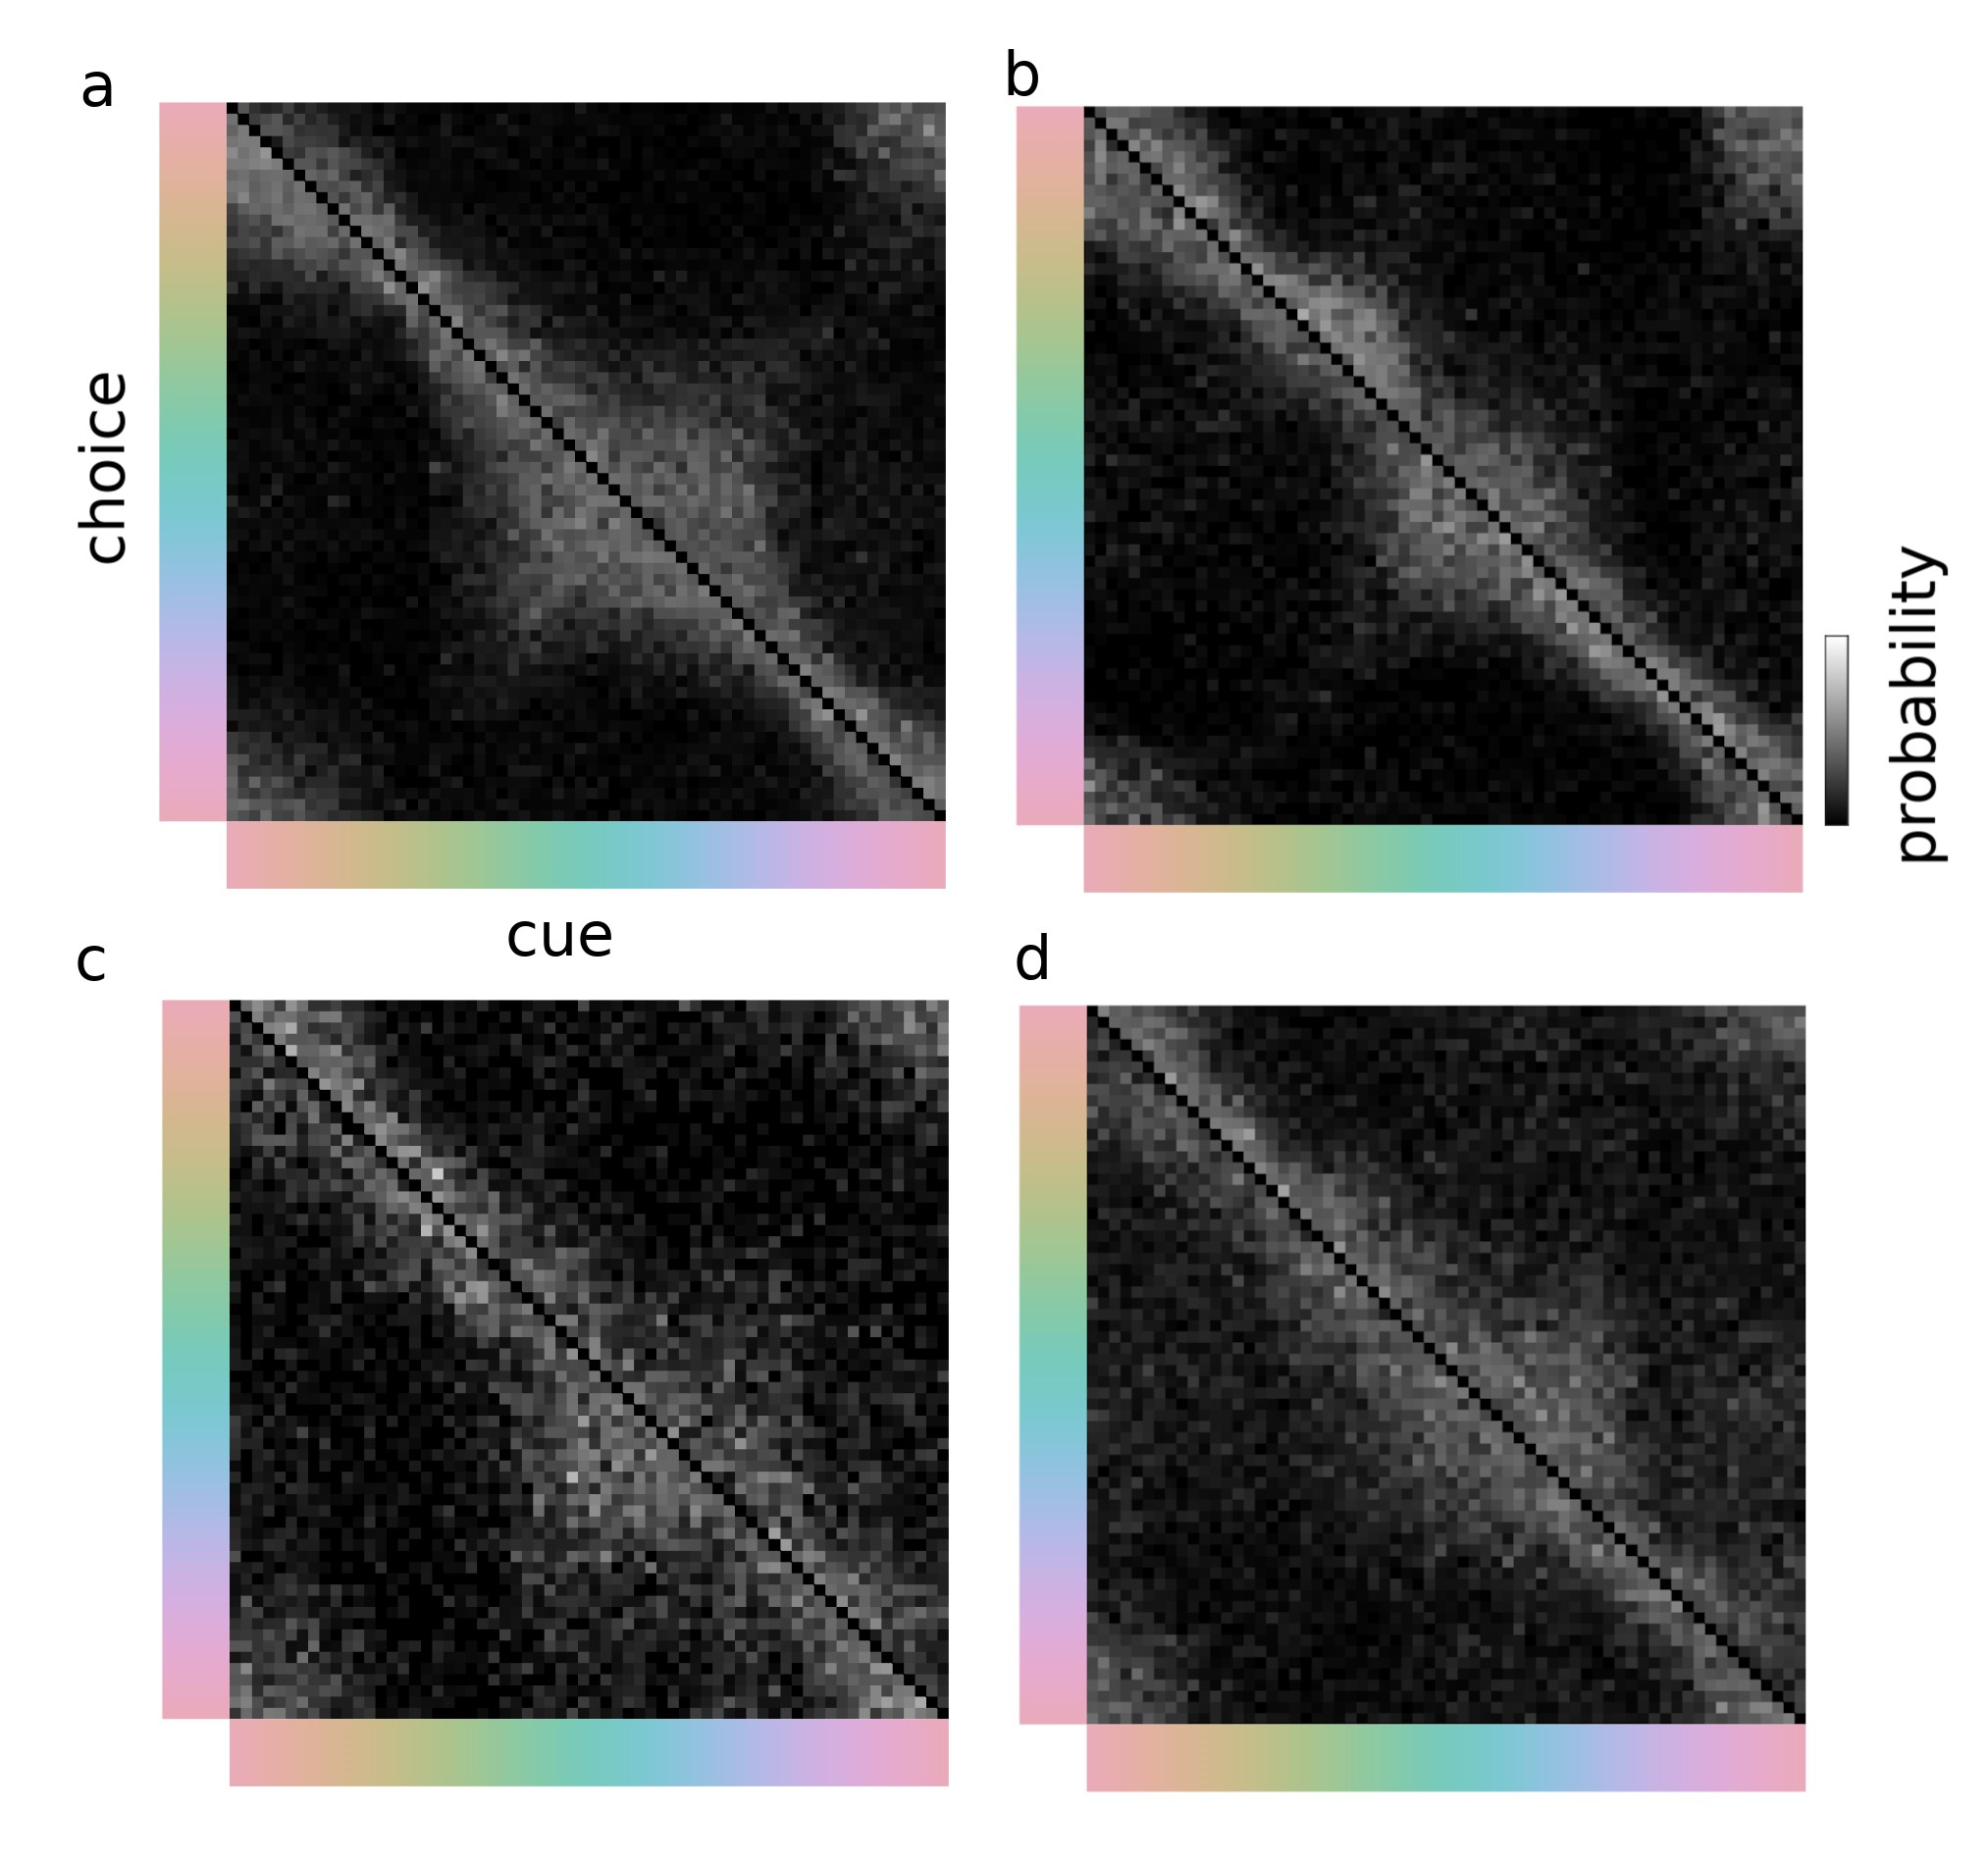
\includegraphics[width=\textwidth+4cm]{../Figures/flat/SI6_choiceMatrices.jpg}
    \caption{\textbf{Choice probability matrices for free similarity matrix models, for the four individuals.}
    As per the similarity matrices presented, each column represents a cue, and each row represents a choice. 
    Here, however, rather than the similarity between cue/choice pairs we show the probability of selection. 
    Whereas the similarity matrix is the output of model fitting, this matrix is derived more directly from the data: each cell is simply the number of times a particular choice was made divided by the number of times that choice was an option. 
    The identity line, representing correct options, is excluded since it is not possible to normalize these values given our paradigm.
    } 
    \label{fig:choiceProbabilityMatrices}
    \end{fullwidth}
\end{figure}

